\documentclass{article}%
\usepackage[T1]{fontenc}%
\usepackage[utf8]{inputenc}%
\usepackage{lmodern}%
\usepackage{textcomp}%
\usepackage{lastpage}%
\usepackage[head=40pt,margin=0.5in,bottom=0.6in]{geometry}%
\usepackage{graphicx}%
%
\title{\textbf{Maduro designa a Adán Chávez como embajador de Venezuela en Cuba}}%
\author{Diario El Universal}%
\date{07/03/2019}%
%
\begin{document}%
\normalsize%
\maketitle%
\textbf{URL: }%
http://www.eluniversal.com/politica/35000/maduro{-}designa{-}a{-}adan{-}chavez{-}como{-}embajador{-}de{-}venezuela{-}en{-}cuba\newline%
%
\textbf{Periodico: }%
EU, %
ID: %
35000, %
Seccion: %
politica\newline%
%
\textbf{Palabras Claves: }%
NO\_TIENE\newline%
%
\textbf{Derecho: }%
2.1%
, Otros Derechos: %
\newline%
%
\textbf{\textit{El dirigente oficialista continuará igualmente como vicepresidente de Asuntos Internacionales del Partido Socialista Unido de Venezuela}}%
\newline%
\newline%
%
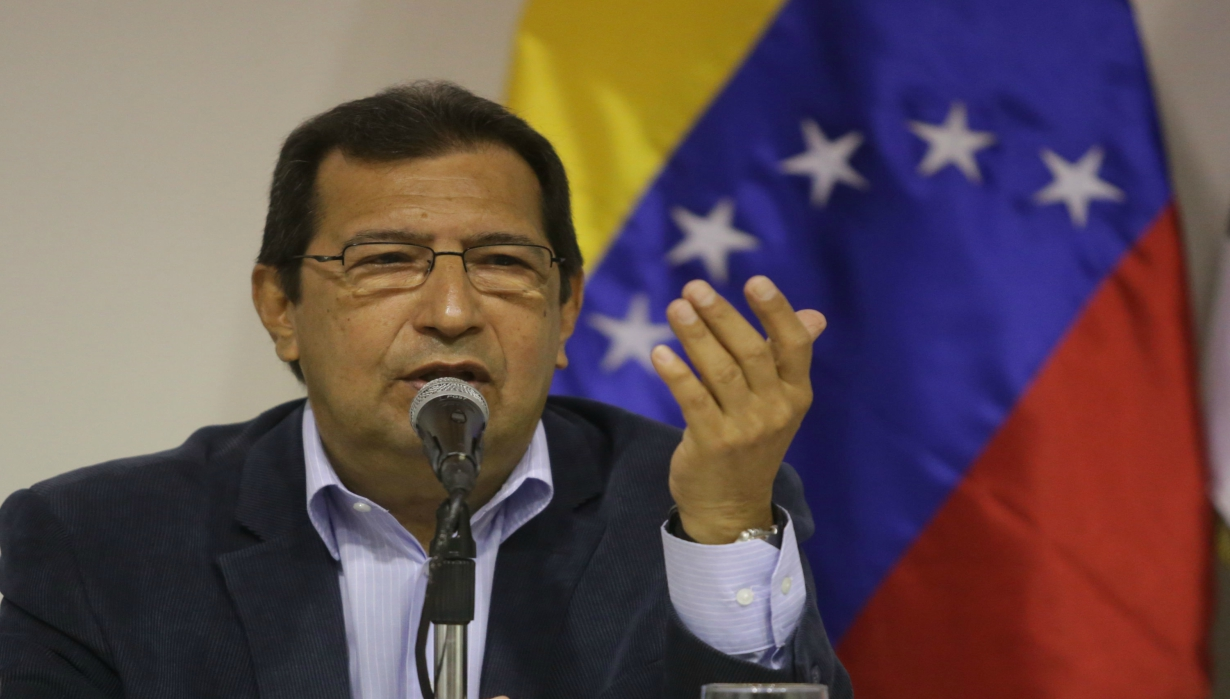
\includegraphics[width=300px]{EU_35000.jpg}%
\newline%
%
Caracas.{-} El gobernante Nicolás Maduro designó a Adán Chávez como embajador de Venezuela en Cuba, quien seguirá igualmente como vicepresidente de Asuntos Internacionales del PSUV.%
\newline%
%
La información la publicó el mandatario a través de su cuenta en la red social Twitter.%
\newline%
%
\end{document}